\section{Virtual Reality Data}
\label{S:t3}
Lack of inclusiveness for pedestrians and, in particular, crossing pedestrians in the available AV datasets raises the need for the exploring dataset specifically designed to account for behavioural patterns of jaywalking and mid-block crossing pedestrians. One solution to achieve such data in a controlled environment, with the possibility of customizing scenarios to include desired conditions, would be to develop and conduct Virtual Reality (VR) experiments. By doing so, and analyzing the behaviour in a controlled, safe, and relatively low-cost environment, we can acquire information on factors determining pedestrian trajectory and provide solutions and suggestions for improving and complementing AV datasets.

For this study, Virtual Immersive Reality Environment (VIRE) is used to simulate different scenarios and conduct experiments on different aspects of pedestrian crossing and walking behaviour. Introduced in~\cite{farooqvire}, VIRE uses Head Mounted Display and virtual reality to enable interactive, immersive and complex simulated scenarios. Hypothetical traffic scenarios can be projected directly to the eyes of users, and with a human-in-the-loop simulation, the behaviour of simulated vehicles is influenced by the behaviour of the participants. In this study, scenarios involve a mid-block crosswalk, with vehicles passing by on the street. Each scenario is designed by a set of variables with different levels designed. Participants wearing the VR headset start on the simulated sidewalk, and in different conditions, are asked to cross the street when they feel it is safe to do so. While doing the experiment, pedestrian reactions, including their coordinates, head orientation and distance to the approaching vehicles are recorded in 0.1-second intervals.   

The data collection campaign was conducted in summer 2018 in four different locations to cover a heterogeneous population. A total of 180 individuals from different age groups participated in the experiment over a period of 5 months. The experiments were performed at Ryerson University, City of Markham Public Library, Toronto City Hall, and North York Civic center. Participants were exposed to multiple scenarios, with changing parameters in each round. In \cref{fig:Texp}, an experiment and its components are shown.
\begin{figure}
\centering
\sbox{\measurebox}{%
  \begin{minipage}[b]{.4\textwidth}
  \subfloat
  {\label{fig:figA}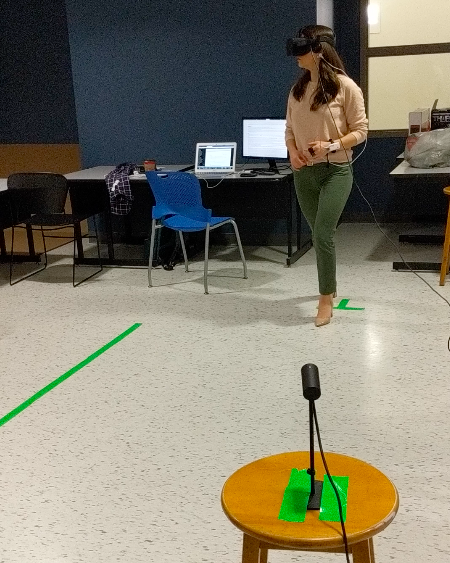
\includegraphics[width=0.91\textwidth,height=8cm]{chapter_6/figures/img1.png}}
    (a)
  \end{minipage}}
\usebox{\measurebox}\qquad
    \begin{minipage}[b][\ht\measurebox][s]{.4\textwidth}
    \centering
    \subfloat
    {\label{fig:figB}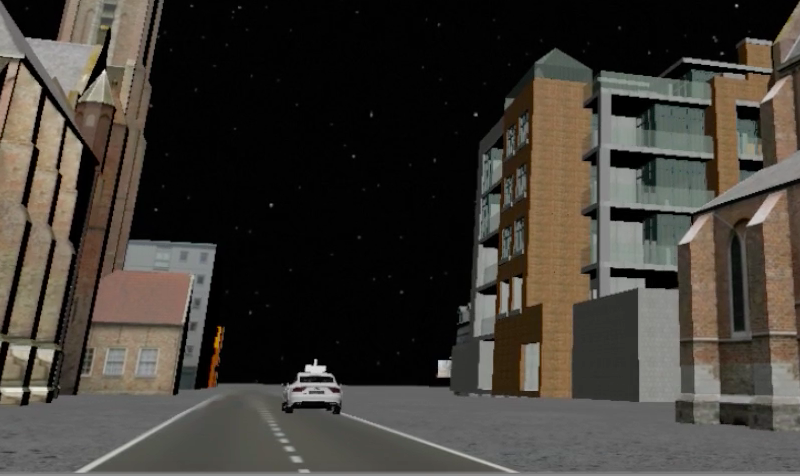
\includegraphics[width=0.91\textwidth,height=3.5cm]{chapter_6/figures/img3.png}}
    (b)
    \vfill
    \subfloat
    {\label{fig:figC}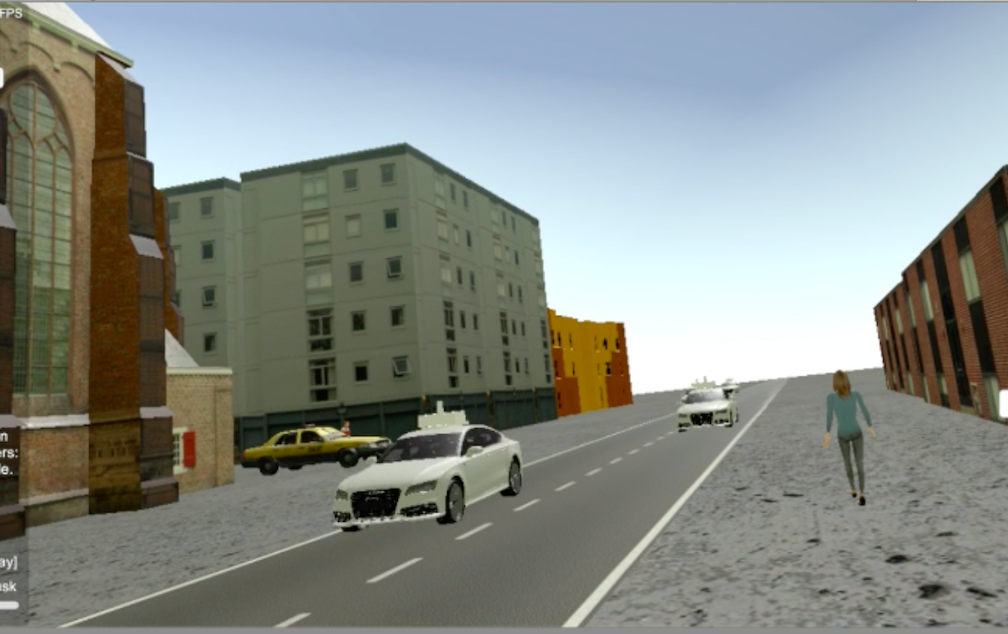
\includegraphics[width=0.91\textwidth,height=3.5cm]{chapter_6/figures/pic1.png}}
    (c)
    \end{minipage}
\caption{VR experiment. (a) A participant doing the experiment (b) A sample night view of the environment (c) A sample day view of the environment}
\label{fig:Texp}
\end{figure}
In addition to recorded time-series data from participants, contextual variables from the the environment of scenarios were captured to include in trajectory prediction models. The environmental context variables include the type of road (one-way, two-way or two-way with median), speed limit (30, 40 or 50 km/hr), lane width (2.5, 2.75 or 3 m), weather conditions (snowy day or clear view), time of the day (day or night), and arrival rate of cars (530, 750, 1100 veh/hr). These variables are selected so that a hypothetical AV can capture and utilize them as input to its trajectory prediction algorithm. Detailed information on the data collection campaign, collected data, scenario details, etc. can be found in ~\cite{kalatian2020decoding}. To concentrate on the interactions of pedestrians with AVs, scenarios involving simulated human-driven vehicles in the traffic are included in this study. Also, other scenario variables that cannot be captured by cameras or LIDAR sensors are not used in the modelling to make sure that a hypothetical AV can deploy the proposed algorithms without requiring information that they cannot capture inherently.